\documentclass[../../../main.tex]{subfiles}
\begin{document}

\subsection{Extrusion nozzle temperature measurement}

Once the needle heating system has been assembled, it is necessary to see how the electrical parameters relate to the actual extruder temperature. 
As mentioned in the previous section, it was decided to leave 3 \textit{mm} of the needle unwound so that the two-wire RTD PT100 thermistor could be used to measure the temperature at the tip. 
As the temperature gradient is negative in the longitudinal direction of the needle, if the temperature at the tip of the needle is equal to the desired temperature, it can be assured that the rest of the needle will also be hotter. 
To use the thermistor, a Wheatstone bridge is required to convert resistance variations into measurable voltage variations. 
As these variations are very small, an amplifier is needed to measure them. 
There are boards with integrated circuits on the market that are used to read the measurements from these sensors. 
These boards integrate the Wheatstone bridge and the amplifier and can be used with Arduino. 
To read the temperature of the thermistor, a MAX31865 amplifier from Adafruit (United States) was purchased.
This amplifier is designed to work with RTD PT100 thermistors. 
The amplifier was integrated into a circuit with an Arduino board, and using code provided by the same company, the voltage could be converted to temperature.

Two different setups were made to measure the tip temperature. 
First, a support was designed to keep the thermistor in direct contact with the lateral surface of the needle, see \cref{fig:setup} \textcolor{blue}{A}. 
Then, in order to measure the temperature at the base of the tip, the thermistor was taped to the bed, and the needle was pressed against the thermistor, see \cref{fig:setup} \textcolor{blue}{B}. 


\begin{figure}[!htbp]
    \centering
    \begin{subfigure}[b]{0.3\textwidth}
        \centering
        \includegraphics[width =\textwidth]{imgs/setup1.pdf}
        \caption{Setup to measure the lateral temperature of the needle.}
     \end{subfigure}
     \hspace{1cm}
    \begin{subfigure}[b]{0.5\textwidth}
        \centering
        \includegraphics[width =\textwidth]{imgs/setup2.pdf}
        \caption{Setup to measure the temperature on the base of the tip.}
     \end{subfigure}
     \caption{Different setups used to measure the temperature of the needle.}
    \label{fig:setup}
\end{figure}

Twenty-one centimetres of Nichrome wire were used to create the coil, which had 25 turns. 
The temperature of the printer hot-block was set to 220$^{\circ}C$. 
The same procedure was followed for both measurements: the voltage was increased by 0.5\textit{V} and after a 10-second wait, the temperature was recorded. 
The first setup was discarded because the contact surface between the thermistor and the needle was too small. 
The thermistor was in more contact with the air than with the needle, and it was not possible to measure the actual temperature. In the \cref{fig:temp_increase} following values recorded in the second setup are shown.

\begin{figure}[!htbp]
\centering
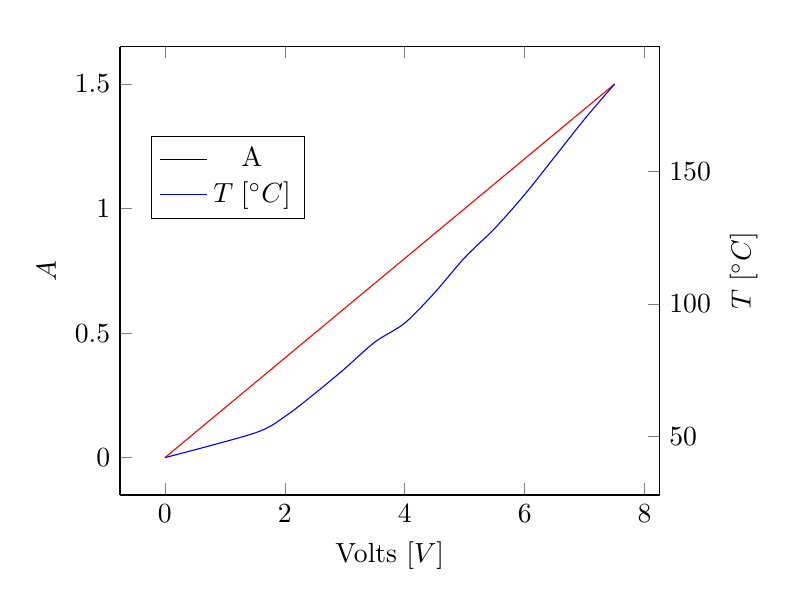
\begin{tikzpicture}
\begin{axis}[
  axis y line*=left,
  axis x line*=bottom,
  xlabel={Volts $[V]$},
  ylabel={$A$},
]
\addplot[smooth,red]
  coordinates{
(0, 0)
(1.5, 0.3)
(2.0, 0.4)
(2.5, 0.5)
(3.0, 0.6)
(3.5, 0.7)
(4.0, 0.8)
(4.5, 0.9)
(5.0, 1.0)
(5.5, 1.1)
(6.0, 1.2)
(6.5, 1.3)
(7.0, 1.4)
(7.5, 1.5)
  }; \label{plot_one}
\end{axis}

\begin{axis}[
  axis y line*=right,
  ylabel={$T\;[^{\circ}C]$},
  ylabel near ticks,
  axis x line*=top,
  xticklabels={},
legend style={at={(0.2,0.8)},anchor=north}
]
\addlegendimage{/pgfplots/refstyle=plot_one}
\addlegendentry{A}
\addplot[smooth,blue]
  coordinates{
    (0, 42)
(1.5, 51.3)
(2.0, 57.5)
(2.5, 66.2)
(3.0, 75.6)
(3.5, 85.6)
(4.0, 92.8)
(4.5, 104.3)
(5.0, 117.5)
(5.5, 128.5)
(6.0, 141.3)
(6.5, 155.5)
(7.0, 169.8)
(7.5, 183)
  };
\addlegendentry{$T\;[^{\circ}C]$}
\end{axis}
\end{tikzpicture}
\caption{Increase in temperature and amperage recorded as a function of the applied voltage.}
\label{fig:temp_increase}
\end{figure}


In addition to the temperature, the amperage values displayed by the power supply were also recorded. 
As can be seen in the figure, the amperage increases linearly with the voltage. 
This indicates that the winding assembly was done correctly, since the variation in the resistance of the nichrome can be assumed to be constant with respect to temperature. 
As for the recorded temperature, it does not increase proportionally to the voltage. 
A change in the slope of the function is observed around 95$^{\circ}C$. 
This may mean that the measurements taken are not reliable. 
In fact, the last temperature recorded was 220.1$^{\circ}C$, reached with 7.5\textit{V} and 1.5\textit{A}.
At the end of the experiment, the polymer was dripping liquid from the extruder, indicating that the actual temperature of the polymer is much higher than 220$^{\circ}C$.
Suspecting that the temperature was not being read correctly, a test was carried out to compare the temperature detected by the printer bed thermistor. 
The plastic bed was removed, and the thermistor was attached to the metal heating plate of the bed. The procedure for this test was similar to the previous one. The bed temperature was increased by 10$^{\circ}C$, and the temperature measured by the thermistor was recorded after 10 seconds. 
The results obtained are shown in \cref{fig:bed_temp}.
It also included the difference of temperatures, $\Delta T$, between the recorded and the set one.
It can be seen that until 90$^{\circ}C$ the difference is less than 3 degrees, but at  90$^{\circ}C$ it increases until a difference of 5$^{\circ}C$ and remains constant until 105$^{\circ}C$, which was the maximum temperature that could be reached on the bed. 
This increase 


\begin{figure}[!htbp]
\centering
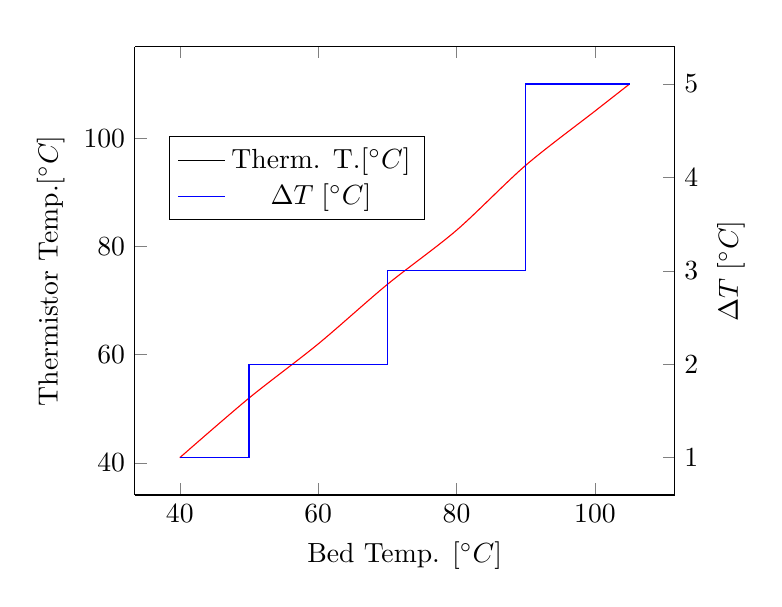
\begin{tikzpicture}
\begin{axis}[
  axis y line*=left,
  axis x line*=bottom,
  xlabel={Bed Temp. [$^{\circ}C$]},
  ylabel={Thermistor Temp.[$^{\circ}C$]},
]
\addplot[smooth,red]
  coordinates{
(40, 41)
(50, 52)
(60, 62)
(70, 73)
(80, 83)
(90, 95)
(100, 105)
(105, 110)
  }; \label{plot_one}
\end{axis}

\begin{axis}[
  axis y line*=right,
  ylabel={$\Delta T\;[^{\circ}C]$},
  ylabel near ticks,
  axis x line*=top,
  xticklabels={},
legend style={at={(0.3,0.8)},anchor=north}
]
\addlegendimage{/pgfplots/refstyle=plot_one}
\addlegendentry{Therm. T.[$^{\circ}C$]}
\addplot[blue]
  coordinates{
(40, 1)
(50,1)
(50, 2)
(60, 2)
(70,2)
(70, 3)
(80, 3)
(90,3)
(90,5)
(90, 5)
(100, 5)
(105, 5)
  };
\addlegendentry{$\Delta T\;[^{\circ}C]$}
\end{axis}
\end{tikzpicture}
\caption{Bed temperature measured by the thermocouple (red) and difference between that temperature and the bed temperature (blue).}
\label{fig:bed_temp}
\end{figure}


This increase in error may be the cause of the change in slope recorded during the reading of extruder temperatures (\cref{fig:temp_increase}). 
Even so, due to the dripping observed at the end of the temperature measurement, it can be assumed that the values obtained are neither reliable nor representative of reality. 
Therefore, it was concluded that it would not be possible to relate the extruder temperature to the electrical parameters.
Then, it was decided to conduct an experimental characterisation of the polymer's rheology to determine the range of electrical parameters that enable the material to be extruded and printed.


\subsection{Electrical characterisation of the heating system}

The purpose of this task is to characterise the extrusion behaviour as a function of electrical parameters. 
As the voltage is higher than the amperage, it was decided to vary the voltage in order to achieve greater precision. 
Therefore, the aim is to find the range of voltage values that make extrusion possible. 
To do this, the same extruder used in the previous section and the same winding will be used. 
The procedure followed was based on applying increments of 0.2\textit{V}, waiting 5 minutes for tempering and extruding 1 \textit{cm} of filament. 
When the extruder is not hot enough and filament is extruded, what happens is that as the filament is solidified inside the tube, the gears that pull the filament slip, emitting a characteristic noise and strong vibration. 

To perform this test, a temperature of 200$^{\circ}C$ was set in the extruder. It was started with a voltage of 1.3\textit{V} and 0.26\textit{A}. 
The first thing that was observed was that when the voltage was kept constant, the amperage fluctuated greatly. 
Therefore, the amperage measurements shown are the average value read over a 5-second interval. 
Using these values, it was possible to extrude a small amount of material, but it solidified quickly, clogging the extruder.
Extrusion was not possible until the current reached 1.9\textit{V}/0.3\textit{A}.
However, with these values, if extrusion stopped at any point, the polymer would cool down again inside the tube. 
From 2.1\textit{V}/0.42\textit{A} onwards, extrusion was maintained even if it stopped, although the molten filament cooled very quickly once it was extruded. 
This suggests that this current reaches the minimum extrusion temperature for PLA, around 180$^{\circ}C$.
Therefore, 0.4\textit{A} was set as the minimum current required for extrusion. 
As the current increased, the polymer was extruded more easily, becoming less viscous, but the effect known as stringing was more noticeable, suggesting that the polymer was heating up significantly.
When a current of 3.3\textit{V}/0.8\textit{A} was reached, spots began to appear on the extruder, indicating that the polymer was burning at some point in the circuit. 
This set the upper current limit at 0.8\textit{A}. Therefore, an amperage between 0.4 and 0.8\textit{A} is required for printing.

\subsection{Preliminary test: planar reference print}

To verify the proper functioning of this customised extruder and the heating system, it was tested by printing a 1 \textit{cm}-side cube. 
The purpose of this test is to show whether it is truly feasible to print using such a long extruder. 
Additionally, it aims to narrow the range of current values even further for use during printing. 
The G-code required to print the cube was generated using UltiMaker Cura 5.9 software. The extruder temperature was 200$^{\circ}C$ and the bed temperature was 60$^{\circ}C$. 
The printing speed was 50 \textit{mm/s} except for the wall printing speed, which was 25 \textit{mm/s}.
The cube was printed with a 30\% infill. 

Starting with applying 0.4\textit{A} of direct current, the cube was printed. 
With this current, the polymer is extruded, but it dries very quickly. 
A skirt-type adhesion plate was printed to improve the adhesion of the first layer, but with this current, the material did not adhere well, and part of the skirt had already come off during printing. 
The same thing happened during printing: the first layers were printed correctly, but at a certain point, the tension of the polymer itself inside the extruder tore off the already printed layers, see \cref{fig:04A}. 
It was observed that the extruded material was less than expected. 
It was also observed that the current varies greatly during printing, reaching values below 0.4\textit{A}.
Due to these current fluctuations, the polymer may not have flowed well, resulting in less extruded material.

\begin{figure}[!htbp]
    \centering
    \includegraphics[width =0.5\textwidth]{imgs/04A.pdf}
    \caption{Cube printing test result with 0.4\textit{A} current.}
    \label{fig:04A}
\end{figure}

The current was increased to 0.5\textit{A}. 
The polymer flows correctly at this current level. 
The quality and quantity of the extrusion during layer printing is good, but the layers at the corners became separated, see \cref{fig:05A}.
Layer decohesion occurs when the printing temperature is low and the polymer cools too quickly. 
Finally, the cube detached from the bed. 
The current continued to fluctuate during printing, as in the previous case, but this time, critical values were not exceeded.

\begin{figure}[!htbp]
    \centering
    \includegraphics[width =0.5\textwidth]{imgs/100vel_05A_vent0.pdf}
    \caption{Cube printing test result with 0.5\textit{A} current.}
    \label{fig:05A}
\end{figure}

The speed was reduced by half while maintaining the current at 0.5\textit{A} to check whether the poor adhesion could be due to the extruder's tension on the printed polymer. 
With these values, the entire cube was successfully printed, but it detached from the bed when the extruder retracted on the last layer. see \cref{fig:05A_2}. 
It can be seen that the print quality is not very promising. 
The corners bent upward, which is a sign of polymer overheating. 
In addition, blobs are visible, which is also a sign of overheating. 
Despite maintaining the same current as in the previous case, the hot extruder now remains in contact with the polymer for much longer once it is printed, due to the speed. 
This excess contact time between the hot tip of the extruder and the polymer seems to overheat it. 
However, despite all this, the entire cube was successfully printed, suggesting that perhaps the printing speed should be lower than initially set.

\begin{figure}[!htbp]
    \centering
    \includegraphics[width =0.5\textwidth]{imgs/50vel_05A_vent0.pdf}
    \caption{Cube printing test result with 0.5\textit{A} current and a printing speed of 25 \textit{mm/s}.}
    \label{fig:05A_2}
\end{figure}

Despite the previous result, adhesion to the bed was not yet satisfactory. 
Therefore, the current was increased to 0.6\textit{A} and the printing speed was maintained at 25 \textit{mm/s}.
The results obtained were the best, see \cref{fig:06A}. 
The piece remained fixed to the base, and the quality of the layers was very good. 
However, the cube was very hot and soft, indicating that the temperature was still too high during printing.

\begin{figure}[!htbp]
    \centering
    \includegraphics[width =0.4\textwidth]{imgs/50vel_06A.pdf}
    \caption{Cube printing test result with 0.6\textit{A} current and a printing speed of 25 \textit{mm/s}.}
    \label{fig:06A}
\end{figure}

To cool the polymer, a 3\textit{W} fan was installed next to the extruder to blow air directly onto the part. 
This was not a solution, as it cooled the extruder too much and caused the polymer inside it to solidify, clogging it up regardless of the power used. 
It was even observed that the fans on the head itself had the capacity to solidify the polymer. 
Therefore, it was concluded that no type of forced cooling could be used.


A final test was carried out by increasing the current to 0.7\textit{A}. 
With this current, it was also possible to print the cube while maintaining adhesion at all stages, see \cref{fig:07A}. 
However, grainy effects were observed, indicating that the polymer had overheated.
It was suspected that this could be due to a possible overflow, so the printing was repeated with a flow rate of 80\% (\cref{fig:07A_2} \textcolor{blue}{A}) and 70\% (\cref{fig:07A_2} \textcolor{blue}{B}). 
The results obtained after these changes were worse, with grains still visible and under-extrusion effects. 
Therefore, it was concluded that the current should be maintained between 0.5\textit{A} and 0.6\textit{A}, and the speed should be relatively low.
To the author's knowledge, at the time of writing this thesis, this is the first hot printing ever performed with such a long extruder.

\begin{figure}[!htbp]
    \centering
    \includegraphics[width =0.5\textwidth]{imgs/50vel_07A.pdf}
    \caption{Cube printing test result with 0.6\textit{A} current and a printing speed of 25 \textit{mm/s}.}
    \label{fig:07A}
\end{figure}


\begin{figure}[!htbp]
    \centering
    \begin{subfigure}[b]{0.32\textwidth}
        \centering
        \includegraphics[width =\textwidth]{imgs/50vel_07A_80FR.pdf}
        \caption{Flow rate = 80\%.}
     \end{subfigure}
     \hspace{1cm}
    \begin{subfigure}[b]{0.3\textwidth}
        \centering
        \includegraphics[width =\textwidth]{imgs/50vel_07A_07FR.pdf}
        \caption{Flow rate = 70\%.}
     \end{subfigure}
     \caption{Assembly of the adapter and the 18-\textit{G} needle}
    \label{fig:07A_2}
\end{figure}


\subsection{Characterisation of printing parameters}

The previous sections have examined the electrical values required to print with this heated extruder. 
This section aims to analyse how printing parameters affect the viability of non-planar printing. 

After several experiments conducted using non-planar printing, it was concluded that the printing parameters that most affect non-planar printing are, a priori, temperature, printing speed, and retraction. 
Therefore, different tests will be performed for each of these parameters. 
The method for conducting these tests will be the same for each parameter: for each value, three vertical columns and three columns inclined at 45$^{\circ}$ will be printed. 
As many rows of columns will be printed, side by side, as there are values to be studied. 
The current used for all the tests was 0.5\textit{A}.


\subsubsection{Temperature test}


The temperature test studied how the temperature of the hot block affects printability. 
To do this, rows were printed at each of the following temperatures: 180, 190, 200 and 210$^{\circ}$.
Before starting to print a column, 0.5 \textit{mm} of material is extruded to improve adhesion to the base. 
The columns were printed at a speed of 10 \textit{mm/s}. 
The printed inclined columns are shown in \cref{fig:temp_test}.

\begin{figure}[!htbp]
    \centering
    \includegraphics[width =\textwidth]{imgs/temp_test.pdf}
    \caption{Inclined columns printed during the temperature test at 180, 190, 200, and 210$^\circ C$ from left to right.}
    \label{fig:temp_test}
\end{figure}

The results obtained show that the temperature of the hot block has practically no effect on printability. 
This result was to be expected, since the temperature that governs printability is that of the tube and not that of the hot block. 
Even so, as can be seen in the image, the last column of the row printed at 180$^{\circ}$ was torn from the base. 
Therefore, it was decided that the printing temperature should be higher than 180$^{\circ}$. 
The intermediate value, 200$^{\circ}$, was chosen from the results as the printing temperature. 
It can also be noticed that all columns have a string of molten polymer on top. 
This phenomenon is known as stringing and is caused by the extruder lifting, see \cref{fig:stringing} \textcolor{blue}{A}. 
To reduce this effect, when the extruder finishes printing a column, it remains stationary for 5 seconds to allow the column to solidify, then rises vertically 1 \textit{cm}, moves to the position of the next column and descends vertically to the starting point of printing. 
Despite this, stringing is inevitable and must be dealt with. 
The problem this can cause is that the extruder can bump into these threads during movement, melting them and causing them to clump together in the extruder, dirtying it and potentially sticking to other already printed parts. 
This could cause tension in the printed parts. 
In \cref{fig:stringing} \textcolor{blue}{B}, it can be seen that despite attempts to reduce its effect, the string can almost double the size of the columns. 

\begin{figure}[!htbp]
    \centering
    \begin{subfigure}[b]{0.4\textwidth}
        \centering
        

% Gradient Info
  
\tikzset {_mzix41zd3/.code = {\pgfsetadditionalshadetransform{ \pgftransformshift{\pgfpoint{0 bp } { 0 bp }  }  \pgftransformrotate{-270 }  \pgftransformscale{2 }  }}}
\pgfdeclarehorizontalshading{_buy4zbb99}{150bp}{rgb(0bp)=(1,1,1);
rgb(54.82142857142857bp)=(1,1,1);
rgb(62.5bp)=(0.61,0.61,0.61);
rgb(100bp)=(0.61,0.61,0.61)}

% Gradient Info
  
\tikzset {_mg3p0nsm3/.code = {\pgfsetadditionalshadetransform{ \pgftransformshift{\pgfpoint{0 bp } { -0.5 bp }  }  \pgftransformrotate{-90 }  \pgftransformscale{2 }  }}}
\pgfdeclarehorizontalshading{_je6tgefoc}{150bp}{rgb(0bp)=(1,1,1);
rgb(37.5bp)=(1,1,1);
rgb(62.5bp)=(0,0,0);
rgb(100bp)=(0,0,0)}
\tikzset{_rhzzu6zch/.code = {\pgfsetadditionalshadetransform{\pgftransformshift{\pgfpoint{0 bp } { -0.5 bp }  }  \pgftransformrotate{-90 }  \pgftransformscale{2 } }}}
\pgfdeclarehorizontalshading{_y9hn7kdjv} {150bp} {color(0bp)=(transparent!0);
color(37.5bp)=(transparent!0);
color(62.5bp)=(transparent!10);
color(100bp)=(transparent!10) } 
\pgfdeclarefading{_vng0zxtvy}{\tikz \fill[shading=_y9hn7kdjv,_rhzzu6zch] (0,0) rectangle (50bp,50bp); } 

% Gradient Info
  
\tikzset {_bj5c9j7rb/.code = {\pgfsetadditionalshadetransform{ \pgftransformshift{\pgfpoint{0 bp } { 0 bp }  }  \pgftransformrotate{-90 }  \pgftransformscale{2 }  }}}
\pgfdeclarehorizontalshading{_qk2kexk1u}{150bp}{rgb(0bp)=(1,0,0);
rgb(49.64285714285714bp)=(1,0,0);
rgb(50.714285714285715bp)=(1,0,0);
rgb(57.23214285714286bp)=(0.29,0.56,0.89);
rgb(100bp)=(0.29,0.56,0.89)}

% Gradient Info
  
\tikzset {_r32u86fl6/.code = {\pgfsetadditionalshadetransform{ \pgftransformshift{\pgfpoint{0 bp } { 0 bp }  }  \pgftransformrotate{-270 }  \pgftransformscale{2 }  }}}
\pgfdeclarehorizontalshading{_hhq9tjtq2}{150bp}{rgb(0bp)=(1,1,1);
rgb(54.82142857142857bp)=(1,1,1);
rgb(62.5bp)=(0.61,0.61,0.61);
rgb(100bp)=(0.61,0.61,0.61)}

% Gradient Info
  
\tikzset {_nkdpehyiu/.code = {\pgfsetadditionalshadetransform{ \pgftransformshift{\pgfpoint{0 bp } { -0.5 bp }  }  \pgftransformrotate{-90 }  \pgftransformscale{2 }  }}}
\pgfdeclarehorizontalshading{_pyxk87nd7}{150bp}{rgb(0bp)=(1,1,1);
rgb(37.5bp)=(1,1,1);
rgb(62.5bp)=(0,0,0);
rgb(100bp)=(0,0,0)}
\tikzset{_mwfa1wyeu/.code = {\pgfsetadditionalshadetransform{\pgftransformshift{\pgfpoint{0 bp } { -0.5 bp }  }  \pgftransformrotate{-90 }  \pgftransformscale{2 } }}}
\pgfdeclarehorizontalshading{_jy97qok0z} {150bp} {color(0bp)=(transparent!0);
color(37.5bp)=(transparent!0);
color(62.5bp)=(transparent!10);
color(100bp)=(transparent!10) } 
\pgfdeclarefading{_wpyz07rb3}{\tikz \fill[shading=_jy97qok0z,_mwfa1wyeu] (0,0) rectangle (50bp,50bp); } 

% Gradient Info
  
\tikzset {_lc7ue9dpu/.code = {\pgfsetadditionalshadetransform{ \pgftransformshift{\pgfpoint{0 bp } { 0 bp }  }  \pgftransformrotate{-90 }  \pgftransformscale{2 }  }}}
\pgfdeclarehorizontalshading{_ayppihpkw}{150bp}{rgb(0bp)=(1,0,0);
rgb(37.5bp)=(1,0,0);
rgb(49.19642857142857bp)=(1,0,0);
rgb(58.125bp)=(0.29,0.56,0.89);
rgb(62.5bp)=(0.29,0.56,0.89);
rgb(100bp)=(0.29,0.56,0.89)}
\tikzset{every picture/.style={line width=0.75pt}} %set default line width to 0.75pt        

\begin{tikzpicture}[x=0.75pt,y=0.75pt,yscale=-1,xscale=1]
%uncomment if require: \path (0,300); %set diagram left start at 0, and has height of 300

%Shape: Square [id:dp10477043116887463] 
\draw  [draw opacity=0][shading=_buy4zbb99,_mzix41zd3] (115,209.33) -- (158,209.33) -- (158,252.33) -- (115,252.33) -- cycle ;
%Shape: Path Data [id:dp6696875766682748] 
\path  [shading=_je6tgefoc,_mg3p0nsm3,path fading= _vng0zxtvy ,fading transform={xshift=2}] (141.7,149.55) -- (133.2,149.55) -- (133.2,70.55) -- (119.7,70.55) -- (119.7,33.55) -- (156.7,33.55) -- (156.7,70.55) -- (141.7,70.55) -- (141.7,149.55) -- cycle ; % for fading 
 \draw   (141.7,149.55) -- (133.2,149.55) -- (133.2,70.55) -- (119.7,70.55) -- (119.7,33.55) -- (156.7,33.55) -- (156.7,70.55) -- (141.7,70.55) -- (141.7,149.55) -- cycle ; % for border 

%Shape: Path Data [id:dp6744062824884621] 
\path  [shading=_qk2kexk1u,_bj5c9j7rb] (141,209.8) -- (134.2,209.8) -- (134.2,66.4) -- (125.4,66.4) -- (125.4,33.8) -- (150,33.8) -- (150,66.4) -- (141,66.4) -- (141,209.8) -- cycle ; % for fading 
 \draw   (141,209.8) -- (134.2,209.8) -- (134.2,66.4) -- (125.4,66.4) -- (125.4,33.8) -- (150,33.8) -- (150,66.4) -- (141,66.4) -- (141,209.8) -- cycle ; % for border 

%Shape: Square [id:dp5760880909889591] 
\draw  [draw opacity=0][shading=_hhq9tjtq2,_r32u86fl6] (206.6,210.53) -- (249.6,210.53) -- (249.6,253.53) -- (206.6,253.53) -- cycle ;
%Shape: Path Data [id:dp31004184155496395] 
\path  [shading=_pyxk87nd7,_nkdpehyiu,path fading= _wpyz07rb3 ,fading transform={xshift=2}] (233.3,131.15) -- (224.8,131.15) -- (224.8,52.15) -- (211.3,52.15) -- (211.3,15.15) -- (248.3,15.15) -- (248.3,52.15) -- (233.3,52.15) -- (233.3,131.15) -- cycle ; % for fading 
 \draw   (233.3,131.15) -- (224.8,131.15) -- (224.8,52.15) -- (211.3,52.15) -- (211.3,15.15) -- (248.3,15.15) -- (248.3,52.15) -- (233.3,52.15) -- (233.3,131.15) -- cycle ; % for border 

%Shape: Path Data [id:dp09202608753864516] 
\path  [shading=_ayppihpkw,_lc7ue9dpu] (233.22,210.31) -- (226.4,210.31) -- (226.4,159.93) .. controls (226.4,159.91) and (226.4,159.9) .. (226.4,159.89) .. controls (226.47,158.49) and (227.89,142.35) .. (228.14,125.98) .. controls (228.39,109.6) and (226.17,96.25) .. (226.14,94.15) -- (226.14,94.15) -- (226.14,94.15) .. controls (226.14,94.14) and (226.14,94.13) .. (226.14,94.12) -- (226.14,48.56) -- (217.59,48.56) -- (217.59,15.22) -- (241.59,15.22) -- (241.59,48.56) -- (232.12,48.56) -- (232.12,94) .. controls (232.12,94.05) and (232.12,94.1) .. (232.12,94.15) .. controls (231.96,96.1) and (231.14,109.6) .. (230.64,126.73) .. controls (230.14,143.85) and (233.22,158.6) .. (233.22,159.89) -- (233.22,210.31) -- cycle ; % for fading 
 \draw   (233.22,210.31) -- (226.4,210.31) -- (226.4,159.93) .. controls (226.4,159.91) and (226.4,159.9) .. (226.4,159.89) .. controls (226.47,158.49) and (227.89,142.35) .. (228.14,125.98) .. controls (228.39,109.6) and (226.17,96.25) .. (226.14,94.15) -- (226.14,94.15) -- (226.14,94.15) .. controls (226.14,94.14) and (226.14,94.13) .. (226.14,94.12) -- (226.14,48.56) -- (217.59,48.56) -- (217.59,15.22) -- (241.59,15.22) -- (241.59,48.56) -- (232.12,48.56) -- (232.12,94) .. controls (232.12,94.05) and (232.12,94.1) .. (232.12,94.15) .. controls (231.96,96.1) and (231.14,109.6) .. (230.64,126.73) .. controls (230.14,143.85) and (233.22,158.6) .. (233.22,159.89) -- (233.22,210.31) -- cycle ; % for border 





\end{tikzpicture}

        \caption{Stringing effect}
     \end{subfigure}
     \hspace{1cm}
    \begin{subfigure}[b]{0.5\textwidth}
        \centering
        \includegraphics[width =\textwidth, angle=270]{imgs/stringing_200C.jpg}
        \caption{Detail of the stringing effect in a vertical column printed at 200$^{\circ}$}
     \end{subfigure}
     \caption{Cause and effect of stringing in non-planar 3D-printing.}
    \label{fig:stringing}
\end{figure}

\subsubsection{Printing speed test}

The objective of the print speed test is to determine the maximum speed at which non-planar printing can be performed without compromising printability. 
Printing speed is directly related to the internal stresses generated when the extruder moves. 
The faster the extruder moves, the less time the polymer has to cool, and therefore the greater the deformation the material will undergo as it leaves the extruder. 
During the test, printing was carried out at the following speeds: 10, 20, 30, 40 and 50 \textit{mm/min}. 
The printing temperature was 200$^{\circ}$.

The speeds chosen for the test were relatively low, and the quality of the prints was similar at different speeds. 
Except for the maximum speed, at which several columns were torn from the bed, and the others suffered deformation. 
\cref{fig:speed_1} and \cref{fig:speed_2} show a comparison between vertical and inclined columns obtained at 10 \textit{mm/min} and 50 \textit{mm/min}.
It can be observed that columns printed at maximum speed are curved in the centre. 
For this reason, printing at speeds greater than or equal to 50 \textit{mm/min} was ruled out. 
It was decided to print at 30 \textit{mm/min} to maintain a certain margin of safety.

\begin{figure}[!htbp]
    \centering
    \begin{subfigure}[b]{0.45\textwidth}
        \centering
        \includegraphics[width =\textwidth, angle=270]{imgs/10S.jpg}
        \caption{Vertical column printed at 10 \textit{mm/min}.}
     \end{subfigure}
    \begin{subfigure}[b]{0.45\textwidth}
        \centering
        \includegraphics[width =\textwidth, angle=270]{imgs/40S.jpg}
        \caption{Vertical column printed at 50 \textit{mm/min}.}
     \end{subfigure}
     \caption{Comparison between two vertical columns printed at 10 and 50 \textit{mm/min} respectively.}
    \label{fig:speed_1}
\end{figure}

\begin{figure}[!htbp]
    \centering
    \begin{subfigure}[b]{0.45\textwidth}
        \centering
        \includegraphics[width =\textwidth, angle=270]{imgs/10S_1.jpg}
        \caption{Inclined column printed at 10 \textit{mm/min}.}
     \end{subfigure}
     \hspace{1cm}
    \begin{subfigure}[b]{0.45\textwidth}
        \centering
        \includegraphics[width = \textwidth, angle=270]{imgs/40S_1.jpg}
        \caption{Inclined column printed at 50 \textit{mm/min}.}
     \end{subfigure}
     \caption{Comparison between two inclined columns printed at 10 and 50 \textit{mm/min} respectively}
    \label{fig:speed_2}
\end{figure}


\subsubsection{Retraction test}

The concept of retraction in 3D printing involves a backwards movement of the filament once extrusion is complete, before the extruder begins to move, to prevent material dripping and the occurrence of stringing.
This test aims to improve the stringing effect experienced during printing. 
To do this, the following retraction values were used: 0, 5, 10, 15, 20, and 25 \textit{mm}. The printing speed was 30 \textit{mm/min} and the temperature was 200$^{\circ}$.
Below is a representative example of each retraction value.

\begin{figure}[!htbp]
    \centering
    \begin{subfigure}[b]{0.35\textwidth}
        \centering
        \includegraphics[width =\textwidth]{imgs/0_5R.pdf}
        \caption{Vertical columns printed with 0 and 5 \textit{mm} retraction, respectively.}
     \end{subfigure}
     \hspace{1cm}
    \begin{subfigure}[b]{0.45\textwidth}
        \centering
        \includegraphics[width = \textwidth]{imgs/0_5R_1.jpg}
        \caption{Inclined columns printed with 0 and 5 \textit{mm} retraction, respectively.}
     \end{subfigure}
     \caption{Comparison between two columns printed with 0 and 5 \textit{mm} retraction.}
    \label{fig:retract_1}
\end{figure}

\begin{figure}[!htbp]
    \centering
    \begin{subfigure}[b]{0.45\textwidth}
        \centering
        \includegraphics[width =\textwidth]{imgs/10_15R.pdf}
        \caption{Vertical columns printed with 10 and 15 \textit{mm} retraction, respectively.}
     \end{subfigure}
     \hspace{1cm}
    \begin{subfigure}[b]{0.43\textwidth}
        \centering
        \includegraphics[width = \textwidth]{imgs/10_15R_1.jpg}
        \caption{Inclined columns printed with 10 and 15 \textit{mm} retraction, respectively.}
     \end{subfigure}
     \caption{Comparison between two columns printed with 10 and 15 \textit{mm} retraction.}
    \label{fig:retract_2}
\end{figure}

\begin{figure}[!htbp]
    \centering
    \begin{subfigure}[b]{0.45\textwidth}
        \centering
        \includegraphics[width =\textwidth]{imgs/20_25R.pdf}
        \caption{Vertical columns printed with 20 and 25 \textit{mm} retraction, respectively.}
     \end{subfigure}
     \hspace{1cm}
    \begin{subfigure}[b]{0.38\textwidth}
        \centering
        \includegraphics[width = \textwidth]{imgs/20_25R_1.jpg}
        \caption{Inclined columns printed with 20 and 25 \textit{mm} retraction, respectively.}
     \end{subfigure}
     \caption[Comparison between two columns printed with 20 and 25 \textit{mm} retraction.]{Comparison between two columns printed with 20 and 25 \textit{mm} retraction.The column on the left in image A lost adhesion during printing and was the only one printed entirely for that retraction value. The column on the right in image A has the previous column attached to it, which was also torn off during printing due to retraction.}
    \label{fig:retract_3}
\end{figure}

Conventionally, the gears that pull the filament are far from the hot block, so the backwards movement they exert on the filament results in internal stresses in the region of the filament where the polymer is melted. 
Due to the high viscosity of the polymer, the molten polymer also tends to move backwards. 
In extruders used for planar printing, the distance between the polymer melting zone and the extrusion hole is usually approximately 1 \textit{cm}. 
In contrast, in the long extruder used, the distance is greater than 6 \textit{cm}. 
This makes the dynamics of the molten polymer very complex to study and predict. 
In addition to the long distance, it is also necessary to take into account the narrow region of the needle where the effects of friction between the fluid and the walls are dominant. 
These two factors significantly affect the polymer's capability to retract. 
As mentioned before, understanding how the polymer behaves inside the customised extruder is a very complex task, so it is only possible to observe the effects and attempt to characterise them. 
In view of the results, it can be deduced that retraction has a very negative effect on extrusion. 
Apparently, the stress applied by the solid polymer on the molten polymer is not sufficient to retract the polymer at the tip. 
What seems to happen instead is that part of the molten polymer near the phase change interface does retract, but the stress information does not travel very far. 
This is possibly due to the high shear stresses experienced by the fluid inside the needle.  
Therefore, part of the pre-chamber located before the needle tube must be drained due to this retraction, and once this retraction is recovered, it is refilled with more molten polymer than there was at the beginning. 
This results in more material in the same space and therefore increases the internal pressure of the polymer. 
This increase in pressure results in an over-extrusion of material. 
Another case observed is that of loss of continuity in the polymer, see \cref{fig:retract_2}. 
This case has been observed at low retraction values. 
What is believed to happen is that, due to the short pulls that the material undergoes, its continuity is lost inside the tube, or that, due to the elongation it undergoes, air may be entering, which, when heated, produces bubbles that favour the discontinuity of the material. 
These conclusions arise after extensive analysis of the behaviour of the polymer under various combinations of different printing and retraction parameters, but they have not been corroborated by simulations or physical-mathematical models. 
Therefore, after extensive testing, it was concluded that retraction does not prevent the effect of stringing and, on the contrary, worsens the quality of the extruded material. 
For this reason, it was decided not to use retraction during printing and to assume that stringing will be present throughout the printing process.
Furthermore, another counterproductive effect of high shrinkage values is that, due to the stresses they generate, many columns were torn from the bed.

\subsubsection{Flow rate test}

Additionally, it was decided to study how the flow rate affected printing, as it was observed that the columns were thicker than the diameter of the extruder, and it was suspected that this parameter might need to be modified to control the amount of extruded material. 
The following flow rate values were used for printing: 1, 0.8, 0.6, 0.4, and 0.2. 
It should be pointed out that the flow rate is a dimensionless parameter that multiplies the extrusion value and serves to vary the amount of material to be extruded with respect to its nominal value. 
Once the columns were printed, the diameter of the verticals was measured.
The results obtained are shown in the \cref{tab:flowrate}.

\begin{table}[!htbp]
\centering
\caption{Column thickness obtained for each flow rate value}
\label{tab:flowrate}
\resizebox{0.5\textwidth}{!}{
\begin{tabular}{c|c}
\hline
\multicolumn{1}{|c|}{\textbf{Flow Rate}} & \multicolumn{1}{c|}{\textbf{Thickness {[}mm{]}}} \\ \hline
1                                        & 1.21 $\pm$ 0.3                                   \\ \hline
0.8                                      & 1.02 $\pm$ 0.2                                   \\ \hline
0.6                                      & 0.96 $\pm$ 0.2                                   \\ \hline
0.4                                      & 0.92 $\pm$ 0.5                                   \\ \hline
0.2                                      & 0.72 $\pm$ 0.1                                   \\ \hline
\end{tabular}
}
\end{table}

It was decided to set a flow rate value equal to 0.7 so that the thickness of the edges to be printed would be 1 \textit{mm}.


\subsection{Non-planar printing tests}

Once the parameters to be used during printing had been decided, non-planar printing tests were carried out to learn about the challenges that may arise and need to be resolved to perform this type of printing. 
As the structures to be printed are reticular structures formed from n-gonal pyramids, it was decided to print regular square pyramids with a base and height of 1 \textit{cm}. 
To improve the adhesion of the edges to the bed, a line is printed connecting all the points of the base of the triangle on which each of the edges will be printed. 
The printing speed used for the base was 800 \textit{mm/min}. 
The hot block temperature was 200$^{\circ}$, the current used was 0.5\textit{A}, the non-planar printing speed was 30 \textit{mm/min}, without retraction, and a flow rate of 70\% was used. 

An initial impression was made with one of the edges of the pyramid in contact with the bed to check whether the base was really necessary. 
\cref{fig:P1} shows two images of the result. 
It can be seen that the edge in contact with the base did not adhere, while the rest did. 
Therefore, it is demonstrated that the base is necessary to improve adhesion.

\begin{figure}[!htbp]
    \centering
    \includegraphics[width =0.6\textwidth]{imgs/P1_no_bed.pdf}
    \caption{Pyramid printed with an incomplete base.}
    \label{fig:P1}
\end{figure}

During subsequent prints, several events were observed that could potentially cause problems at some point during printing. 
The first of these, as mentioned in the previous section, is the accumulation of molten polymer on the needle as a result of stringing, which can cause collisions and tension in the printed parts. 
\cref{fig:prob1} \textcolor{blue}{A} shows how these threads stick to the extruder and accumulate, increasing its thickness. 
Furthermore, it is not only the threads resulting from stringing that cause material to accumulate in the extruder. 
As can be seen in \cref{fig:prob1} \textcolor{blue}{B}, near the top vertex of the pyramids, the extruder ends up touching the already printed parts. 
As the extruder is very hot, it tends to remelt the solidified polymer on the adjacent edges, causing it to stick to the tip. 
This causes the extruder to increase in thickness and become dirty, and also removes material from the already printed parts, modifying their topology. 
The first problem has already been mentioned as unavoidable. 
The second can be reduced by modifying the printing trajectories, ending the printing of an edge at the point where the extruder is about to collide with others. 
The problem with this solution is that it can lead to situations where the edges do not converge at any point. 
During testing, it was observed that the part of the extruder that actually contacts the edges is the area free of winding, so it is at a lower temperature. 
However, this may not be the case with different extruders or pyramid configurations. 

\begin{figure}[!htbp]
    \centering
    \begin{subfigure}[b]{0.465\textwidth}
        \centering
        \includegraphics[width =\textwidth]{imgs/stringing_detail_1.pdf}
        \caption{Detail of strings glued and melted on the tip.}
     \end{subfigure}
     \hspace{1cm}
    \begin{subfigure}[b]{0.36\textwidth}
        \centering
        \includegraphics[width = \textwidth]{imgs/detalle_aguja_tocando_2.pdf}
        \caption{Detail of the extruder colliding with already printed edges, melting them.}
     \end{subfigure}
     \caption{Problems detected during the initial pyramids printings.}
    \label{fig:prob1}
\end{figure}

The following problem observed is related to the previous one mentioned. 
The extruder will inevitably collide with the edges at the top, as this area is where all the edge volumes intersect. 
What ends up happening is that when the extruder comes into contact with the printed edges, it melts them and bends them upwards. 
However, it does not melt them enough for them to join together, so it only deforms them upwards. 
\cref{fig:prob2} shows two cases where this occurs. 
In one of them, the top of the edges is bent upwards, but they are joined together, and in the other, they have separated due to the deformation they have undergone. 
In addition to this, when an edge is finished being extruded and the extruder is lifted, some of the material inside the extruder sticks to the edge, making it slightly longer than it actually is. 
The material is not cut at the tip of the extruder but inside it. 
The presence of this excess material causes the position of the node to change. 
Since the node is located at the point of convergence of the edges, this point is displaced upwards, which cannot be predicted, forcing the starting point of the upper edges to be modified. 

\begin{figure}[!htbp]
    \centering
    \begin{subfigure}[b]{0.41\textwidth}
        \centering
        \includegraphics[width =\textwidth]{imgs/Detalle punta 1.jpg}
        \caption{Pyramid with the top ends connected.}
     \end{subfigure}
     \hspace{1cm}
    \begin{subfigure}[b]{0.45\textwidth}
        \centering
        \includegraphics[width = \textwidth]{imgs/puntas_abiertas.pdf}
        \caption{Pyramid with separated top points.}
     \end{subfigure}
     \caption{Pyramids with deformations at their upper vertices due to the extruder colliding at the intersection points of the edges.}
    \label{fig:prob2}
\end{figure}

To solve this problem, it was proposed to print only the non-intersecting volumes of each of the edges of each pyramid. 
To calculate the point up to which each edge should be printed, the intersection of all the 1 \textit{mm} section cylinders that make up the pyramid is calculated, and the intersection point with the lowest \textit{z} coordinate is obtained. 
Once calculated, the upper vertex of an edge will be the point within the set of points that make up an edge whose \textit{z}-coordinate is equal to the minimum obtained from the intersection. 
\cref{fig:intersect} shows a diagram illustrating an example of the proposed solution. 
In the example, the intersection between the two cylinders is shown, delimited by a red triangle. 
And within this intersection, the point with the lowest \textit{z}-coordinate is the point marked as $I_{z_{m}{}_{i}{}_{n}}$. 
Therefore, all edges will be printed up to that coordinate. 
In the example, this point is denoted as $x_2'$ and is obtained using the expression provided in the example. 
Once the cut edges have been printed, the extruder moves to the vertex position and, after waiting 5 seconds, extrudes 1 \textit{mm} of material. 
The purpose of the waiting time is to allow the extruder to melt the printed surfaces before extruding, thereby facilitating the adhesion of the extruded material to the material that has already solidified.

\begin{figure}[!htbp]
    \centering
    

% Gradient Info
  
\tikzset {_6asfs7uar/.code = {\pgfsetadditionalshadetransform{ \pgftransformshift{\pgfpoint{0 bp } { 0 bp }  }  \pgftransformrotate{0 }  \pgftransformscale{2 }  }}}
\pgfdeclarehorizontalshading{_tzbw14iea}{150bp}{rgb(0bp)=(0.65,0.81,0.87);
rgb(37.5bp)=(0.65,0.81,0.87);
rgb(62.5bp)=(0.14,0.33,0.54);
rgb(100bp)=(0.14,0.33,0.54)}

% Gradient Info
  
\tikzset {_btbdxkyxl/.code = {\pgfsetadditionalshadetransform{ \pgftransformshift{\pgfpoint{0 bp } { 0 bp }  }  \pgftransformrotate{0 }  \pgftransformscale{2 }  }}}
\pgfdeclarehorizontalshading{_8qi4bynkf}{150bp}{rgb(0bp)=(0.65,0.81,0.87);
rgb(37.5bp)=(0.65,0.81,0.87);
rgb(62.5bp)=(0.14,0.33,0.54);
rgb(100bp)=(0.14,0.33,0.54)}

% Pattern Info
 
\tikzset{
pattern size/.store in=\mcSize, 
pattern size = 5pt,
pattern thickness/.store in=\mcThickness, 
pattern thickness = 0.3pt,
pattern radius/.store in=\mcRadius, 
pattern radius = 1pt}
\makeatletter
\pgfutil@ifundefined{pgf@pattern@name@_8wfg0k71t}{
\pgfdeclarepatternformonly[\mcThickness,\mcSize]{_8wfg0k71t}
{\pgfqpoint{0pt}{0pt}}
{\pgfpoint{\mcSize+\mcThickness}{\mcSize+\mcThickness}}
{\pgfpoint{\mcSize}{\mcSize}}
{
\pgfsetcolor{\tikz@pattern@color}
\pgfsetlinewidth{\mcThickness}
\pgfpathmoveto{\pgfqpoint{0pt}{0pt}}
\pgfpathlineto{\pgfpoint{\mcSize+\mcThickness}{\mcSize+\mcThickness}}
\pgfusepath{stroke}
}}
\makeatother

% Pattern Info
 
\tikzset{
pattern size/.store in=\mcSize, 
pattern size = 5pt,
pattern thickness/.store in=\mcThickness, 
pattern thickness = 0.3pt,
pattern radius/.store in=\mcRadius, 
pattern radius = 1pt}
\makeatletter
\pgfutil@ifundefined{pgf@pattern@name@_xnv7yu27c}{
\pgfdeclarepatternformonly[\mcThickness,\mcSize]{_xnv7yu27c}
{\pgfqpoint{0pt}{-\mcThickness}}
{\pgfpoint{\mcSize}{\mcSize}}
{\pgfpoint{\mcSize}{\mcSize}}
{
\pgfsetcolor{\tikz@pattern@color}
\pgfsetlinewidth{\mcThickness}
\pgfpathmoveto{\pgfqpoint{0pt}{\mcSize}}
\pgfpathlineto{\pgfpoint{\mcSize+\mcThickness}{-\mcThickness}}
\pgfusepath{stroke}
}}
\makeatother
\tikzset{every picture/.style={line width=0.75pt}} %set default line width to 0.75pt        

\begin{tikzpicture}[x=0.75pt,y=0.75pt,yscale=-1,xscale=1]
%uncomment if require: \path (0,300); %set diagram left start at 0, and has height of 300

%Shape: Parallelogram [id:dp6533548986011148] 
\path  [shading=_tzbw14iea,_6asfs7uar] (259.5,99.25) -- (300.5,99.25) -- (247.5,212.25) -- (206.5,212.25) -- cycle ; % for fading 
 \draw   (259.5,99.25) -- (300.5,99.25) -- (247.5,212.25) -- (206.5,212.25) -- cycle ; % for border 

%Shape: Parallelogram [id:dp34560458612152767] 
\path  [shading=_8qi4bynkf,_btbdxkyxl] (299.98,99.25) -- (342,99.25) -- (410.07,213.13) -- (368.04,213.13) -- cycle ; % for fading 
 \draw   (299.98,99.25) -- (342,99.25) -- (410.07,213.13) -- (368.04,213.13) -- cycle ; % for border 

%Shape: Parallelogram [id:dp8059552336289659] 
\draw  [pattern=_8wfg0k71t,pattern size=6pt,pattern thickness=0.75pt,pattern radius=0pt, pattern color={rgb, 255:red, 0; green, 0; blue, 0}] (277.98,62.25) -- (318.9,62.25) -- (300.5,99.25) -- (259.58,99.25) -- cycle ;
%Shape: Parallelogram [id:dp0629718517202077] 
\draw  [pattern=_xnv7yu27c,pattern size=6pt,pattern thickness=0.75pt,pattern radius=0pt, pattern color={rgb, 255:red, 0; green, 0; blue, 0}] (278.35,62.13) -- (319.67,62.13) -- (341.82,99.25) -- (300.5,99.25) -- cycle ;
%Shape: Triangle [id:dp7200105034736191] 
\draw  [color={rgb, 255:red, 255; green, 0; blue, 0 }  ,draw opacity=1 ][dash pattern={on 4.5pt off 4.5pt}] (300.5,99.42) -- (277.98,62.25) -- (318.9,62.25) -- cycle ;
%Straight Lines [id:da9672903240875802] 
\draw    (301,150.92) -- (301,108.42) ;
\draw [shift={(301,106.42)}, rotate = 90] [color={rgb, 255:red, 0; green, 0; blue, 0 }  ][line width=0.75]    (10.93,-3.29) .. controls (6.95,-1.4) and (3.31,-0.3) .. (0,0) .. controls (3.31,0.3) and (6.95,1.4) .. (10.93,3.29)   ;
%Straight Lines [id:da3736787116789462] 
\draw [color={rgb, 255:red, 255; green, 0; blue, 0 }  ,draw opacity=1 ] [dash pattern={on 4.5pt off 4.5pt}]  (238.67,99.33) -- (368,99.5) ;
%Shape: Circle [id:dp5393133473174121] 
\draw  [color={rgb, 255:red, 255; green, 3; blue, 3 }  ,draw opacity=1 ][fill={rgb, 255:red, 255; green, 0; blue, 0 }  ,fill opacity=1 ] (297.67,99.42) .. controls (297.67,97.85) and (298.94,96.58) .. (300.5,96.58) .. controls (302.06,96.58) and (303.33,97.85) .. (303.33,99.42) .. controls (303.33,100.98) and (302.06,102.25) .. (300.5,102.25) .. controls (298.94,102.25) and (297.67,100.98) .. (297.67,99.42) -- cycle ;
%Shape: Circle [id:dp2526287800180739] 
\draw  [color={rgb, 255:red, 0; green, 0; blue, 0 }  ,draw opacity=1 ][fill={rgb, 255:red, 0; green, 0; blue, 0 }  ,fill opacity=1 ] (297,62.42) .. controls (297,60.85) and (298.27,59.58) .. (299.83,59.58) .. controls (301.4,59.58) and (302.67,60.85) .. (302.67,62.42) .. controls (302.67,63.98) and (301.4,65.25) .. (299.83,65.25) .. controls (298.27,65.25) and (297,63.98) .. (297,62.42) -- cycle ;
%Shape: Circle [id:dp9672546021067726] 
\draw  [color={rgb, 255:red, 0; green, 0; blue, 0 }  ,draw opacity=1 ][fill={rgb, 255:red, 0; green, 0; blue, 0 }  ,fill opacity=1 ] (384.67,213.08) .. controls (384.67,211.52) and (385.94,210.25) .. (387.5,210.25) .. controls (389.06,210.25) and (390.33,211.52) .. (390.33,213.08) .. controls (390.33,214.65) and (389.06,215.92) .. (387.5,215.92) .. controls (385.94,215.92) and (384.67,214.65) .. (384.67,213.08) -- cycle ;
%Straight Lines [id:da2019049632137535] 
\draw    (206,216.5) -- (248.33,216.17) ;
\draw [shift={(248.33,216.17)}, rotate = 179.55] [color={rgb, 255:red, 0; green, 0; blue, 0 }  ][line width=0.75]    (0,3.35) -- (0,-3.35)(6.56,-1.97) .. controls (4.17,-0.84) and (1.99,-0.18) .. (0,0) .. controls (1.99,0.18) and (4.17,0.84) .. (6.56,1.97)   ;
\draw [shift={(206,216.5)}, rotate = 359.55] [color={rgb, 255:red, 0; green, 0; blue, 0 }  ][line width=0.75]    (0,3.35) -- (0,-3.35)(6.56,-1.97) .. controls (4.17,-0.84) and (1.99,-0.18) .. (0,0) .. controls (1.99,0.18) and (4.17,0.84) .. (6.56,1.97)   ;
%Straight Lines [id:da6795988079967963] 
\draw    (272.33,59.5) -- (200.83,211.25) ;
\draw [shift={(200.83,211.25)}, rotate = 295.23] [color={rgb, 255:red, 0; green, 0; blue, 0 }  ][line width=0.75]    (0,3.35) -- (0,-3.35)(6.56,-1.97) .. controls (4.17,-0.84) and (1.99,-0.18) .. (0,0) .. controls (1.99,0.18) and (4.17,0.84) .. (6.56,1.97)   ;
\draw [shift={(272.33,59.5)}, rotate = 115.23] [color={rgb, 255:red, 0; green, 0; blue, 0 }  ][line width=0.75]    (0,3.35) -- (0,-3.35)(6.56,-1.97) .. controls (4.17,-0.84) and (1.99,-0.18) .. (0,0) .. controls (1.99,0.18) and (4.17,0.84) .. (6.56,1.97)   ;
%Shape: Circle [id:dp16058383762793094] 
\draw  [color={rgb, 255:red, 0; green, 0; blue, 0 }  ,draw opacity=1 ][fill={rgb, 255:red, 0; green, 0; blue, 0 }  ,fill opacity=1 ] (318.67,99.08) .. controls (318.67,97.52) and (319.94,96.25) .. (321.5,96.25) .. controls (323.06,96.25) and (324.33,97.52) .. (324.33,99.08) .. controls (324.33,100.65) and (323.06,101.92) .. (321.5,101.92) .. controls (319.94,101.92) and (318.67,100.65) .. (318.67,99.08) -- cycle ;

% Text Node
\draw (290.17,151.83) node [anchor=north west][inner sep=0.75pt]  [font=\scriptsize] [align=left] {$\displaystyle I_{z_{m}{}_{i}{}_{n}}$};
% Text Node
\draw (294.5,41.33) node [anchor=north west][inner sep=0.75pt]  [font=\footnotesize] [align=left] {$\displaystyle x_{2}$};
% Text Node
\draw (392.33,216.08) node [anchor=north west][inner sep=0.75pt]  [font=\footnotesize] [align=left] {$\displaystyle x_{1}$};
% Text Node
\draw (221.67,220.33) node [anchor=north west][inner sep=0.75pt]  [font=\footnotesize] [align=left] {$\displaystyle d$};
% Text Node
\draw (218.47,129.25) node [anchor=north west][inner sep=0.75pt]  [font=\footnotesize,rotate=-295.73] [align=left] {$\displaystyle L$};
% Text Node
\draw (340,79.67) node [anchor=north west][inner sep=0.75pt]  [font=\footnotesize] [align=left] {$\displaystyle x_{2} '$};
% Text Node
\draw (408.33,94.33) node [anchor=north west][inner sep=0.75pt]   [align=left] {$\displaystyle x_{2} '\ =\ x_{2} -\dfrac{\| I_{z_{m}{}_{i}{}_{n}} \ -\ x_{2} \| }{L} \cdotp \overrightarrow{( x_{2} -x_{1})}$};


\end{tikzpicture}

    \caption{Pyramid printed with an incomplete base.}
    \label{fig:intersect}
\end{figure}

\begin{figure}[!htbp]
    \centering
    \begin{subfigure}[b]{0.41\textwidth}
        \centering
        \includegraphics[width =\textwidth]{imgs/Detalle punta 1.jpg}
        \caption{Pyramid with the top ends connected.}
     \end{subfigure}
     \hspace{1cm}
    \begin{subfigure}[b]{0.45\textwidth}
        \centering
        \includegraphics[width = \textwidth]{imgs/puntas_abiertas.pdf}
        \caption{Pyramid with separated top points.}
     \end{subfigure}
     \caption{Result of the process of trimming the edges at the point of intersection and depositing 1 mm of material.}
    \label{fig:prob2}
\end{figure}

\cref{fig:sol1} shows two perspectives of a printed pyramid with trimmed edges. 
It can be seen that the edges no longer match and that there is still residual material at the tip due to the extruder's lifting. 
\cref{fig:sol2} shows two pyramids printed after the entire process mentioned above. 
With this solution, a joined and homogeneous vertex is obtained. 
Therefore, this procedure will be used when generating the G-code for printing future structures. 

\begin{figure}[!htbp]
    \centering
    \begin{subfigure}[b]{0.46\textwidth}
        \centering
        \includegraphics[width =\textwidth]{imgs/detalle_punta_2.pdf}
     \end{subfigure}
     \hspace{1cm}
    \begin{subfigure}[b]{0.35\textwidth}
        \centering
        \includegraphics[width = \textwidth]{imgs/detalle_punta_sol_2.pdf}
     \end{subfigure}
     \caption{Pyramids with trimmed edges.}
    \label{fig:sol1}
\end{figure}

\begin{figure}[!htbp]
    \centering
    \begin{subfigure}[b]{0.43\textwidth}
        \centering
        \includegraphics[width =\textwidth]{imgs/P3_1.pdf}
     \end{subfigure}
     \hspace{1cm}
    \begin{subfigure}[b]{0.45\textwidth}
        \centering
        \includegraphics[width = \textwidth]{imgs/P3_2.pdf}
     \end{subfigure}
     \caption{Pyramids with deformations at their upper vertices due to the extruder colliding at the intersection points of the edges.}
    \label{fig:sol2}
\end{figure}

\subsection{Non-planar printing of the first layer of tetrahedral structures}

Once the electrical and printing parameters that offer the best printability have been obtained and a procedure for printing each of the tetrahedra has been established, the next step is to verify that the viability shown during the tests is maintained when printing more complex structures. 
To achieve this, the first layer of tetrahedra was extracted from a cylinder 4 \textit{cm} wide and 6 \textit{cm} high, which had a high porosity. 
The first layer of tetrahedra will always be composed of pyramids and is therefore easier to print. 
In this case, the layer consists of 28 pyramids with an average height of 9.65 \textit{mm} (min 6.3 \textit{mm} and max 15.8 \textit{mm}). 
The edges that form part of the base, added to improve the adhesion of the structure to the bed, are shown in cyan blue. 
This base is printed in a planar manner, and the paths used to print it are obtained by means of a Depth-First Search to minimise the number of times it is lifted from the extruder and, therefore, stringing on the base.

\begin{figure}[!htbp]
    \centering
    \includegraphics[width= 0.6\textwidth]{imgs/first_layer.pdf}
    \caption{Illustration of the first layer of pyramids obtained from a 4 \textit{cm} wide and 6 \textit{cm} high cylinder. A base was added to increase the adhesion between the printed parts and the bed, shown in cyan.}
    \label{fig:first_layer}
\end{figure}

The printing parameters utilised during the test are shown in \cref{tab:tetra_test_params}. 
Additionally, a layer height of 50\% of the extruder's width was set, and two layers of the base were printed.
\begin{table}[!htbp]
\centering
\caption{Parameters utilised during the first layer test printing.}
\label{tab:tetra_test_params}
\resizebox{0.5\textwidth}{!}{%
\begin{tabular}{c|c}
\hline
\textbf{Current {[}\textit{A}{]}}                        & 0.5  \\ \hline
\textbf{Hot-end temperature {[}$^{\circ}$\textit{C}{]}}            & 200  \\ \hline
\textbf{Bed temperature {[}$^{\circ}$\textit{C}{]}}                & 60   \\ \hline
\textbf{Planar printing speed {[}\textit{mm/min}{]}}     & 9000 \\ \hline
\textbf{Non-planar printing speed {[}\textit{mm/min}{]}} & 20   \\ \hline
\textbf{Retraction {[}\textit{cm}{]}}                    & 0    \\ \hline
\textbf{Flow rate}                              & 0.7  \\ \hline
\end{tabular}%
}
\end{table}

During the initial tests, several problems were observed. 
The first of these was a lack of adhesion between the printed parts and those being printed. 
This problem is particularly significant at the base of the edges, where they rest on the base. 
Various solutions were tested to improve adhesion at the base of the edges. 
Initially, before printing an edge, 0.5 \textit{mm} of polymer was extruded to create a base for the edge and increase the contact area with the bottom parts. 
This was not sufficient, as for some reason, the extra material was not always extruded, see \cref{fig:test_prob1}. 
An attempt was then made to start printing the edges from inside the base. 
To do this, the extruder penetrated the last layer of the base to a distance of half the layer height. 
This ended up damaging the base and was therefore discarded.
Furthermore, this solution could only be used on the first layer of tetrahedra. 
However, it was observed that melting the solidified polymer with the extruder before extrusion improved the adhesion between the two surfaces. 
Therefore, it was decided to return to the initial procedure but add a 5-second pause before starting extrusion so that the extruder, in contact with the solidified polymer, would melt the polymer of the base. 


\begin{figure}[!htbp]
    \centering
    \includegraphics[width= 0.6\textwidth]{imgs/detail_base_adhesion.pdf}
    \caption{Example case of the problem of poor adhesion between edges and the base. Two edges are shown that have poor adhesion to the base. The edge where the contact area between the edge and the base is very small, impairing adhesion, is highlighted with a circle. The other edge collapsed due to this lack of adhesion. A line is included to show the theoretical position of this edge.}
    \label{fig:test_prob1}
\end{figure}

The next issue observed is that when the extruder begins to print an edge that starts at a node from which an edge has already been printed, it melts the base of the printed edge, often tearing it off. 
\cref{fig:test_prob2} shows a sequence of this issue where an already printed edge is torn off.
This problem is critical as it directly affects the viability of the structure. 


\begin{figure}[!htbp]
    \centering
    \begin{subfigure}[b]{0.3\textwidth}
        \includegraphics[width = \textwidth]{imgs/prob2_1.pdf}
     \end{subfigure}
    \begin{subfigure}[b]{0.3\textwidth}
        \includegraphics[width =\textwidth]{imgs/prob2_2.pdf}
     \end{subfigure}
     \begin{subfigure}[b]{0.3\textwidth}
        \includegraphics[width =\textwidth]{imgs/prob2_3.pdf}
     \end{subfigure}
     \caption{Sequence of a previously printed edge being torn off due to the extruder colliding with it when printing a new edge that converges at the same node as the previous one.}
    \label{fig:test_prob2}
\end{figure}


To solve it, a similar approach was taken to that used to improve the connection of the edges at the vertices. 
For each of the nodes, the intersection between all the edges is calculated, and the highest vertical coordinate of this intersection is obtained with the intention of printing a semi-sphere with a radius equal to this coordinate at the node. 
This eliminates all the space where the extruder would collide with the printed edges and also improves the adhesion of the base of the edges.  
After implementing this latest solution, another problem was observed, which highlighted an intrinsic issue with the extruder. 
It was noted that there was a problem with the extrusion of the polymer. 
The extrusion is not continuous or constant, but irregular and variable.
\cref{fig:test_prob3} shows a sequence of the formation of these discontinuities. 
It can be seen that more than the required amount is extruded at one point, which means that there is no material left to extrude afterwards.
Additionally, it was observed that after a certain amount of time printing, darkened areas began to appear on the filament, see \cref{fig:test_prob3_2} \textcolor{blue}{B}.
In light of this, it was decided to halt the tests to study the possible causes of this irregular extrusion in more depth, as it was considered a very critical problem.

\begin{figure}[!htbp]
    \centering
    \begin{subfigure}[b]{0.45\textwidth}
        \includegraphics[width = \textwidth]{imgs/blob_1.pdf}
     \end{subfigure}
    \begin{subfigure}[b]{0.445\textwidth}
        \includegraphics[width =\textwidth]{imgs/blob_2.pdf}
     \end{subfigure}

     \caption{Sequence of formation of a discontinuity during the extrusion of an edge.}
    \label{fig:test_prob3}
\end{figure}


\begin{figure}[!htbp]
    \centering
    \begin{subfigure}[b]{0.42\textwidth}
        \includegraphics[width = \textwidth]{imgs/prob3_1.pdf}
        \caption{Example of material overextrusion}
     \end{subfigure}
    \begin{subfigure}[b]{0.51\textwidth}
        \includegraphics[width =\textwidth]{imgs/prob3_2.pdf}
        \caption{Detail of blackened areas after printing.}
     \end{subfigure}

     \caption{Detail of printing errors. Image A shows an example of over-extrusion during the printing of a tetrahedron. Figure B shows a detail of edges that have blackened during printing.}
    \label{fig:test_prob3_2}
\end{figure}

\subsection{Analysis of the behaviour of the extrusion process}

During printing tests, it was observed that extrusion became unstable after a period of time. 
This inconsistency directly affects the viability of printing and needs to be addressed. 
The effects observed were both over-extrusion and under-extrusion of material. 
No recurring situation was observed that could be the cause of these discontinuities. 
Therefore, it was ruled out that it could be a G-code error. 
It should be noted that retraction was not used during printing. 
Consequently, a thorough analysis of the extrusion behaviour was initiated.
Before the analysis was carried out, the extruder assembly was replaced with a completely new one to rule out assembly problems with the previous ones.

The first potential problem observed is related to the extruder assembly. 
It was noted that molten polymer leaks from the joints between the needle and the adapter. 
\cref{fig:leaking} \textcolor{blue}{A} shows an image of the condition of a recently assembled extruder after extruding material for some time. 
It can be seen that there are polymer leaks at the aforementioned joints despite having ensured that the moving parts were as tight as possible. 
After a longer period of time, the material continued to leak until it covered the entire needle with molten polymer, see \cref{fig:leaking} \textcolor{blue}{B}. 
The leakage of material may be a cause of the discontinuities present in the extrusion. 
However, the leaked material does not represent a large volume of polymer and occurs over time. 
Therefore, it should not cause a total interruption of the flow, but rather a reduction in it, and there must be another cause that has a greater effect on the extrusion. 

\begin{figure}[!htbp]
    \centering
    \begin{subfigure}[b]{0.5\textwidth}
        \includegraphics[width = \textwidth]{imgs/leaking_1.pdf}
        \caption{Leaking material at the joints of the extruder highlighted with red circles.}
     \end{subfigure}
     \hspace{1cm}
    \begin{subfigure}[b]{0.313\textwidth}
        \includegraphics[width =\textwidth]{imgs/leaking_2.pdf}
        \caption{Leaking material after a long period of extrusion.}
     \end{subfigure}

     \caption{Leakage of molten polymer through the extruder joints during extrusion.}
    \label{fig:leaking}
\end{figure}

The leakage of material may be due to the design of the extruder. 
As mentioned above, the Luer lock does not completely prevent longitudinal slippage of the needle. 
The high internal pressure of the molten polymer appears to be pushing the needle forward. 
It was observed that the needle even rotated due to the pressure, indicating that the internal pressure is so high that it manages to unscrew the needle slightly and that at a certain point the thread locks the needle in place, preventing it from coming loose. 
Due to this loosening of the needle, gaps may be created through which the material can escape. 
As for the material leaking at the junction with the hot block, it is unknown why this is happening, as this junction should be watertight. 
The fact that this leak is occurring indicates that this is not actually the case and that there are gaps through which material may be leaking. 
Even if the thread on the adapter were as long as the thread on the hot block, the nut itself should prevent material from leaking. 
It should be noted that material leakage in this area was only observed with the customised extruder, thus ruling out any possible problem with the hot block. 

In addition, it was observed that after a period of printing, the material that leaked was grey in colour, which drew attention to the overheating of the polymer at some point in the extrusion assembly.
Furthermore, the fact that the material can leak indicates that its viscosity has been greatly reduced due to high temperature, allowing it to flow. 
These situations led to a focus on the state of the polymer during extrusion. 
Technically, the material should not overheat, as extrusion was carried out at 200$^\circ C$ and 0.5\textit{A}. 
These values had previously been verified as compatible with correct printing. 
However, the tests to characterise the printing parameters lasted between 10 and 30 minutes, while the printing of the first layer of tetrahedra took more than 1 hour.
Therefore, the polymer could have overheated due to prolonged exposure to heat sources.
To verify this, filament was extruded at the same speed as during printing, 20 \textit{mm/min}. 
After approximately 10 minutes of operation, it was observed that the extruded polymer had roughness, see \cref{fig:hotfil} \textcolor{blue}{A}. 
After 25 minutes, this roughness became more prominent, even deforming the extruded filament, \cref{fig:hotfil} \textcolor{blue}{B}. 
The presence of roughness in the extruded material is usually due to the presence of moisture inside the filament. 
After heating, the water contained within the filament evaporates, creating bubbles that burst and cause pitting. 
To check if this was the case, the filament was replaced with a new one, but the roughness appeared even with the new filament. 
Therefore, it was ruled out that moisture was causing this problem. 
It was hypothesised that the polymer itself was overheating at some point, causing localised evaporation.

\begin{figure}[!htbp]
    \centering
    \begin{subfigure}[b]{0.3\textwidth}
        \includegraphics[width = \textwidth]{imgs/hotfil_1.pdf}
        \caption{Roughness present on the filament after 10 minutes of extrusion.}
     \end{subfigure}
     \hspace{1cm}
    \begin{subfigure}[b]{0.3\textwidth}
        \includegraphics[width =\textwidth]{imgs/hotfil_2.pdf}
        \caption{Roughness present on the filament after 25 minutes of extrusion.}
     \end{subfigure}

     \caption{Example of inconsistencies observed in the filament after different periods of operation.}
    \label{fig:hotfil}
\end{figure}

To find any potential hot spots that might be causing the problem, the tip was removed and extruded using only the adapter. 
It was observed that the roughness continued to appear, see \cref{fig:hotfil_2} \textcolor{blue}{A}. 
Therefore, the adapter was also removed and extruded without the adapter to rule out any possible damage inside the printer's hot block. 
Once the adapter was removed, the roughness stopped appearing, \cref{fig:hotfil_2} \textcolor{blue}{A}. 
It was therefore concluded that the problem was with the adapter. 
To discard any machining problems that might be inside the conduit in the adapter, the adapter was placed back on, the printing temperature was lowered to 180$^\circ C$, and extrusion was performed. 
This time, the extruded filament did not show any roughness. 
Therefore, it was concluded that the roughness could not be caused by poor machining of the adapter. 
In view of this, the hypothesis that hot spots were being generated gained strength. 
This was further reinforced when it was observed that after extruding with the adapter for a while, blackened areas began to appear on the extruded filament, \cref{fig:hotfil_2} \textcolor{blue}{B}. 
This could be an indication that the filament is burning at some point. 
The hot spots could not be found, nor could their appearance be accounted for. 
The hypothesis is that the adapter thread does not reach the end of its stroke, leaving an area where the polymer is in contact with the hot block, see \cref{fig:sec}. 
The hot block may be at a higher temperature than indicated by the thermocouple, as long as the extruder is at the desired temperature. 
And it may be that this temperature is sufficient to burn the polymer. 
In addition, as the printing speed is so low, the time during which the polymer would be in contact with the hot block would be long. 
This could heat it to a temperature sufficient for bubbles to form. Once formed, these bubbles travel through the extruder. 
If the bubbles reach a large size, they can travel through the extruder, obstructing the needle and affecting the continuity of the extruded material. 
This is why edges are observed where part of them is directly missing. 
If they are smaller, they can restrict the flow of material, causing a local decrease in it.
Also, as the heat block is made of aluminium, it has greater thermal conductivity than the adapter, which is made of brass. 
This causes the adapter to retain heat better and increase the temperature of the filament even more, to the point where it can burn it.
In addition to this hot spot, it is believed that the chamber created at the entrance to the needle tube, due to the design of the needle, can also help to create hot spots where the material reaches even higher temperatures. 
Due to the temperature limits found in the tests, the temperature of the hot block cannot be lowered enough to prevent this from happening. 
Furthermore, lowering the temperature does not solve the problem, but only delays it. 
The problem is essentially due to the design of the extruder.
Since the use of this extrusion assembly was the only remaining solution for non-planar printing at high temperatures, it was decided to abandon the improvement of non-planar printing until an adapter with a correct design for use with the hot block could be found. 
Alternatively, a threaded needle that would allow printing without the need for an adapter could be used. 

\begin{figure}[!htbp]
    \centering
    \begin{subfigure}[t]{0.47\textwidth}
        \includegraphics[width = \textwidth]{imgs/hotfil_5.pdf}
        \caption{Comparison of extruded filament without adapter (left) and with adapter (right).}
     \end{subfigure}
     \hspace{1cm}
    \begin{subfigure}[t]{0.415\textwidth}
        \includegraphics[width =\textwidth]{imgs/hotfil_6.pdf}
        \caption{Fragments of filament extruded with the adapter. Burned areas can be seen in the central piece.}
     \end{subfigure}

     \caption{A) Effect of the adapter's presence on the extruded material. B) Effects of polymer overheating after prolonged periods of extrusion.}
    \label{fig:hotfil_2}
\end{figure}

\begin{figure}[!htbp]
    \centering
    \begin{subfigure}[t]{0.35\textwidth}
        \includegraphics[width = \textwidth]{imgs/sec_2.pdf}
        \caption{Conventional assembly.}
     \end{subfigure}
     \hspace{1cm}
    \begin{subfigure}[t]{0.4\textwidth}
        \includegraphics[width =\textwidth]{imgs/sec_1.pdf}
        \caption{Assembly with the extruder using a shorter nut, creating a gap between the extruder and the heat break.}
     \end{subfigure}

     \caption{Cross section of the hot block of a conventional 3D printer. The heat break is shown in blue, the aluminium resistive block in red, and the extruder in orange.}
    \label{fig:sec}
\end{figure}


\end{document}